\documentclass{article}
\usepackage{tabularx}
\usepackage{amsmath}
\usepackage{amssymb}
\usepackage{tikz}
\usetikzlibrary{timeline}
\usepackage{booktabs}
\usepackage{float}
\restylefloat{table}
\graphicspath{{images/}}
\usepackage[margin={1.5cm,2cm}]{geometry}
\usepackage{multicol}
\setlength\columnsep{1.5cm}
\usepackage{tabto}
\usepackage{pdflscape}
\usepackage{graphicx}
\usepackage{array}
\usepackage[T1]{fontenc}
\usepackage[utf8]{inputenc}
\usepackage{charter}
\usepackage{environ}
\usepackage{tikz}
\usetikzlibrary{calc,matrix}
% For citations
\usepackage[sort,numbers]{StyFiles/natbib}
\renewcommand{\citename}{\citet}
\renewcommand{\cite}{\citep}
\usepackage{StyFiles/natbibspacing}


% code by Andrew:
% http://tex.stackexchange.com/a/28452/13304
\makeatletter
\let\matamp=&
\catcode`\&=13
\makeatletter
\def&{\iftikz@is@matrix
  \pgfmatrixnextcell
  \else
  \matamp
  \fi}
\makeatother

\newcounter{lines}
\def\endlr{\stepcounter{lines}\\}

\newcounter{vtml}
\setcounter{vtml}{0}

\newif\ifvtimelinetitle
\newif\ifvtimebottomline
\tikzset{description/.style={
  column 2/.append style={#1}
 },
 timeline color/.store in=\vtmlcolor,
 timeline color=red!80!black,
 timeline color st/.style={fill=\vtmlcolor,draw=\vtmlcolor},
 use timeline header/.is if=vtimelinetitle,
 use timeline header=false,
 add bottom line/.is if=vtimebottomline,
 add bottom line=false,
 timeline title/.store in=\vtimelinetitle,
 timeline title={},
 line offset/.store in=\lineoffset,
 line offset=4pt,
}

\NewEnviron{vtimeline}[1][]{%
\setcounter{lines}{1}%
\stepcounter{vtml}%
\begin{tikzpicture}[column 1/.style={anchor=east},
 column 2/.style={anchor=west},
 text depth=0pt,text height=1ex,
 row sep=1ex,
 column sep=1em,
 #1
]
\matrix(vtimeline\thevtml)[matrix of nodes]{\BODY};
\pgfmathtruncatemacro\endmtx{\thelines-1}
\path[timeline color st] 
($(vtimeline\thevtml-1-1.north east)!0.5!(vtimeline\thevtml-1-2.north west)$)--
($(vtimeline\thevtml-\endmtx-1.south east)!0.5!(vtimeline\thevtml-\endmtx-2.south west)$);
\foreach \x in {1,...,\endmtx}{
 \node[circle,timeline color st, inner sep=0.15pt, draw=white, thick] 
 (vtimeline\thevtml-c-\x) at 
 ($(vtimeline\thevtml-\x-1.east)!0.5!(vtimeline\thevtml-\x-2.west)$){};
 \draw[timeline color st](vtimeline\thevtml-c-\x.west)--++(-3pt,0);
 }
 \ifvtimelinetitle%
  \draw[timeline color st]([yshift=\lineoffset]vtimeline\thevtml.north west)--
  ([yshift=\lineoffset]vtimeline\thevtml.north east);
  \node[anchor=west,yshift=16pt,font=\large]
   at (vtimeline\thevtml-1-1.north west) 
   {\textsc{Timeline \thevtml}: \textit{\vtimelinetitle}};
 \else%
  \relax%
 \fi%
 \ifvtimebottomline%
   \draw[timeline color st]([yshift=-\lineoffset]vtimeline\thevtml.south west)--
  ([yshift=-\lineoffset]vtimeline\thevtml.south east);
 \else%
   \relax%
 \fi%
\end{tikzpicture}
}

\begin{document}
\begin{titlepage}
	\centering
	\begin{figure}[H]
	\centering
	%\includegraphics[scale=0.5]{logo_nasa_trio_black@2x.png}
	\end{figure}
	\vspace{2cm}
	{\scshape\LARGE Ph.D. Research Proposal\par}
	\vspace{2cm}
	{\scshape\LARGE Interpretative Sequence Learning Under Deep
    Learning \& Graphical Model Framework \par}
	{\huge\bfseries \par}
	
	\vspace{2cm}
	{\Large\itshape Chang Li\par}
	\vfill
	{\Large\itshape Supervisor\par}
	{\Large\itshape Prof. Dacheng \textsc{Tao}\par}
	\vfill

\end{titlepage}
\section{Objective}

\begin{itemize}
	\item Potentially discovering rare forms of radio sources by classification in different classes.
	\item Reduction in time to generate scientific results by radio astronomers.
	\item Deeper insight into topological representation of radio data during classification.
\end{itemize}


\section{Introduction}
\subsection{Morphological Classes of Radio Galaxies}

Radio galaxies with active nuclei can be distinguished based on their radio luminosity or brightness of their radio emissions in relation to their hosting environment. Some of the basic morphological classifications include point sources, extended sources i.e. sources with extended contours, double radio sources, jets, and lobes.


\subsection{Problems faced with current classification}

Currently Radio astronomers manually classify galaxies based on visual inspection of the images which is a slow procedure, and increases the time to production of scientific results. Further, it introduces uncertainities in the classification procedure, both of which are problems which can potentially be mitigated by using an automated approach.

Contemporary algorithms classify radio sources into at most three different classes. Our aim is to build a robust model capable of handling more than 2 classes.

\section{Approach}

\subsection{Source Modelling}
  The first step would be source extraction using the standard technique of gaussian modelling. We propose to do this using the robust PyBDSM pipeline used for fitting gaussian distributions to radio sources. The software contains a plethora of features, from which we would be using a small subset. This would mainly include:

\begin{enumerate}
\item Source extraction using gaussian modelling of radio data.
\item Generation of a catalog file containing details of radio sources (RA, DEC, Size of Gaussian (min, max), etc.)
\end{enumerate}

\subsection{Cutout Generation}
The second step would be to convert the RA(Right Ascension) and DEC (Declination) values generated from the catalog, to their corresponding pixel values in the original image. Based on these pixel values we generate 10*10 px cutouts using as reference the co-ordinates of the center of the radio source. This involves a multistep procedure briefly including:
\begin{enumerate}
\item Reading the FITS image in the form of a matrix
\item Parsing through the generated catalog file and extracting data for each radio source such as RA, DEC, etc.
\item Converting the RA and DEC values from WCS (World Coordinate System) to pixel values.
\item Processing pixel values to account for difference in addressing between FORTRAN and C family of languages.
\item Slicing the image matrix assuming the reference pixel co-ordinates as the center of the source.
\end{enumerate}

Prototype code for section \textit{3.1} and section \textit{3.2} has been written mainly for testing purposes. We used a sample image from the TGSS survey which was then processed using the first two steps of our pipeline to generate 470 cutout images.
More details can be found at: 
https://github.com/NCRA-TIFR/radiogen.

\subsection{Data Preprocessing}

Real world data is incomplete, inconsistent and noisy. Techniques like data cleaning, integration, transformation, reduction, discretization are required to ensure data uniformity.

Standard techniques include:
\begin{enumerate}
\item Mean Subtraction 

The mean is subtracted across every feature in the data cloud. The geometric interpretation of this operation is the centering of the data cloud around the origin along every dimension.

\item Normalization

The data dimensions to span the same range. This results in higher accuracy during data processing, as inter-dimensional variance is accounted for. There are two common ways of achieving this normalization. 
\begin{enumerate}
\item Divide each dimension by its standard deviation, once it has been zero-centered.
\item Normalize each dimension to result in a range of values [-1,1].
\end{enumerate}
\begin{figure}[H]
\centering
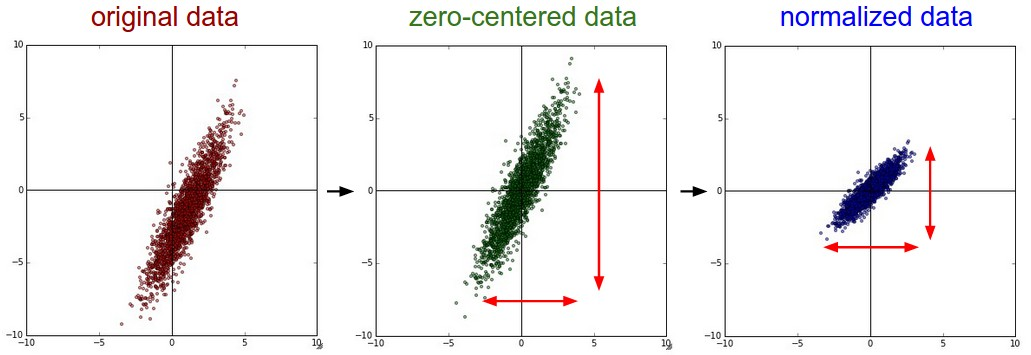
\includegraphics[scale=0.26]{prepro1.jpeg}
\caption{Mean Subtraction and Normalization}
\end{figure}

\item Dimensionality Reduction using Principal Component Analysis

The main linear technique for dimensionality reduction, principal component analysis, performs a linear mapping of the data to a lower-dimensional space in such a way that the variance of the data in the low-dimensional representation is maximized. By finding the eigen vector with the highest eigen value we select the Principal component axis with the highest variance and the minimum reconstruction error. Dimension reduction occurs by eliminating axes with eigen vectors exhibiting the least variance.
This results in a data representation exhibiting a higher degree of variance, leading to faster convergence and greater accuracy during classification.

\begin{figure}[H]
\centering
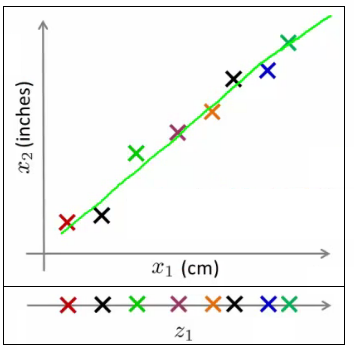
\includegraphics[scale=0.75]{pca.png}
\caption{Reduction from 2D to 1D using PCA}
\end{figure}
\end{enumerate}
\subsection{Analytical Approach}
The analytical approach to solving the problem of galaxy morphology classification would primarily contain two steps:
\begin{enumerate}
\item Feature extraction using sophisticated techniques prevalent in image processing.
\item Building a statistical model of the extracted features
\item Cross comparison of the designed model with principal indicators of dominant classes
\end{enumerate}
A variety of techniques have been used to tackle the related problem of visual recognition in Computer Vision. The standard algorithm for feature extraction is the Scale Invariant Feature Transform (SIFT).

\subsubsection{Scale Invariant Feature Transform} 
The SIFT algorithm extracts keypoints from a set of reference images and stores them in a database. The feature vectors of the extracted images are compared wih the reference vectors on the basis of a defined norm (usually Euclidean distance). The probability that of the subset of features indicating the presence of an object is computed. This gives the accuracy of the fit. When multiple features pass these tests, the class can be correctly identified with a high confidence.
\begin{figure}[H]
\centering
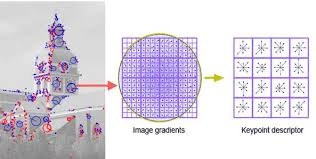
\includegraphics[scale=0.75]{sift.jpg}
\caption{Feature Extraction using SIFT}
\end{figure}

\subsection{Empirical Approach}

An empirical approach is a way of gaining knowledge by means of direct and indirect observation or experience. In the context of this project, we plan to employ Artificial Neural Networks(ANNs), which are a computational model based on a large collection of artifical neurons, that learn hierarchical representations of the data. Each neural unit is connected with many other units which computes to essentially create a non-linear stacked function approximator. Neural networks typically consist of multiple layers in which a signal traverses from the input layer to the output layer.

A convolutional neural network (CNN), is a type of ANN, is a state of the art model that currently provide the best solutions to many problems in computer vision such as  image segmentation, recognition and classification\cite{alex}.

Convolutional neural networks were designed to use minimal amounts of preprocessing. A typical architecture of a CNN consists of convolutional layers, activation layers and pooling layers each of which is briefly explained.
\begin{itemize}
\item Convolution layer:
Performs the convolution operation with a static filter on input from previous layers.
\item Activation layer: 
Defines the output of a unit given an input or set of inputs by applying an activation function. 
\item Pooling layer: 
Progressively reduces the spatial size of the representation, which results in a decreased number of parameters and thus reduction in network computation.
\end{itemize}    
The initial layers of the CNNs learn simple features in the input data such as straight edges, simple colors, and curves. The deeper layers learn the higher level representation of image and search for complex shapes and structures. Mathematically, deeper layers can be thought of as compositions of previous layers. \cite{alex}\cite{Zeiler}\cite{karparthy}. 

\begin{figure}[H]
\centering
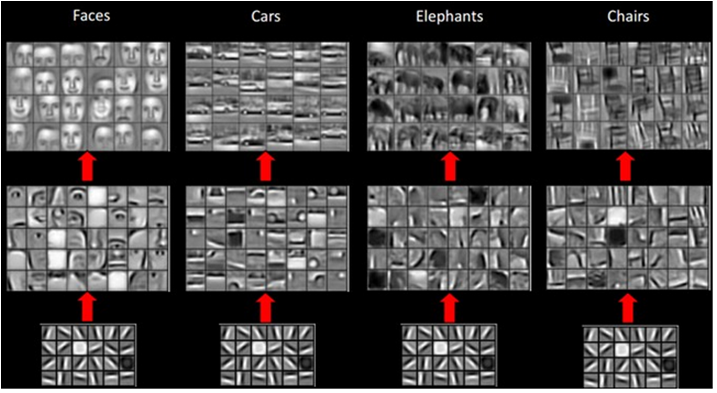
\includegraphics[scale=1.5]{cnn.png}
\caption{CNN learning simple features on initial layers for different classes}
\end{figure}

Variants of CNNs have achieved great successes for morphological galaxy classification and prediction on SDSS\cite{Sander}. Sander Dieleman et al. won the Galaxy challenge, an international competition on Kaggle, to build the best model for morphology
classication based on annotated images from the Galaxy Zoo project.

\section{Timeline}

\begin{vtimeline}[timeline color=cyan!80!blue, line offset=2pt]
April - May & Literature survey\endlr
Mid-August to September & Hypothesis testing \endlr
September to October & Prototype implementation\endlr
October to November & System refinement\endlr
November to December & Publishing results\endlr
\end{vtimeline}

\section{Conclusion}

We would like to thank Dr.Yogesh Wadadekar
\footnote{\label{NCRA-TIFR} National Center for Radio
  Astrophysics - Tata Institute of Fundamental Research}, Dr.C.
H. Ishwara Chandra for their
supportive presence during the process of brainstorming potential
research ideas. Their constant guidance has been an invaluable
source of inspiration for us, and we are eager to continue
working with them.
\bibliographystyle{abbrvnat}
\bibliography{proposal.bib}
\end{document}
